\documentclass[11pt,letterpaper]{exam}
%\usepackage[Lhdr={},Rhdr={}]{plain}

\newtheorem{proposition}{Proposition}
\newcommand{\blue}[1]{\textcolor{blue}{#1}}
\newcommand{\white}[1]{\textcolor{white}{#1}}

\usepackage{tikz}
\usetikzlibrary{shapes.geometric}
\usepackage{pgfplots}
\usetikzlibrary{patterns, pgfplots.fillbetween}
\usepackage{graphicx}
\usepackage{verbatim}
\usepackage{subfigure}
\usetikzlibrary{positioning}
\usetikzlibrary{snakes}
\usetikzlibrary{calc}
\usetikzlibrary{arrows}
\usetikzlibrary{decorations.markings}
\usetikzlibrary{shapes.misc}
\usetikzlibrary{matrix,shapes,arrows,fit,tikzmark}
\usepackage{amsmath}
\usepackage{mathpazo}
\usepackage{hyperref}
\usepackage{lipsum}
\usepackage{multimedia}
\usepackage{graphicx}
\usepackage{multirow}
\usepackage{graphicx}
\usepackage{dcolumn}
\usepackage{bbm}
\usepackage{comment}
 \usepackage{booktabs}
\usepackage{tabularx}
\usepackage{adjustbox}
\usepackage{graphicx}
\usepackage{multicol}
\usepackage{mathtools}
\usepackage[table,xcdraw]{xcolor}
\usepackage[top=0.5in,
  headsep=0pt% remove space between header and text body
  ]{geometry}
\usepackage{lastpage}
\cfoot{Page \thepage \hspace{1pt} of \pageref{LastPage}}

\newcommand{\figpath}{figs/}

\usepackage{titlesec}
\titleformat*{\section}{\large\bfseries}

\begin{document}
\begin{center}
\Large{\textsc{International Trade Theory and Policy}}\\[4pt]
\Large{ECON 2181 \;--\; Fall 2025}\\[6pt]
\large Carlos Góes, Ph.D. \\
\textit{Professorial Lecturer}\\
\href{mailto:c.bezerradegoes@gwu.edu}{c.bezerradegoes@gwu.edu} \\
\end{center}

\bigskip

\begin{center}
\Large{\textsc{Problem Set 2}}
\end{center}


\begin{questions}

\question   Consider a world with 2 countries $i \in \{ H, F\}$ and multiple goods indexed by $g \in [0,1]$. In country $i$, there are $L_i$ units of labor (worker-hours) available, which we call the labor endowment. An inherent technological characteristic of country $i$ are \textbf{unit labor requirements}, i.e. to produce one unit of good $g$ firms in country $i$ use $a_{i,g}$ units of labor. In country $i$, firms producing good $g$ maximize profits under perfect competition. Assume there are no shipping costs across countries.

\begin{parts}
\part  Write down the profit maximization function of firm producing good $g$ in country $i$. Assume firms take prices $P_g$ as given. Give and economic interpretation to each term in the function the firm maximizes.
\textcolor{red}{
        \begin{equation*}\label{eq: production}
            \max_{Y_{i,g}} \pi_{i,g} = \max_{Y_{i,g}} \underbrace{P_{g}Y_{i,g}}_{\text{total revenues}} - \underbrace{w_i a_{i,g} Y_{i,g}}_{\text{total costs}} 
        \end{equation*}
}

\part  Recall that in perfect competition profits for each good are equal to zero. Given that information, express the price of good $P_g$ as a function of cost of production. Give an economic interpretation for the result.

\textcolor{red}{
        \begin{equation*}
             P_{g}Y_{i,g} -  w_i a_{i,g} Y_{i,g} = 0 \implies P_g = w_i a_{i,g}
        \end{equation*}
}
\textcolor{red}{ perfect competition, prices equal marginal cost (how many workers are necessary to produce one unit $a_{i,g}$ times how much you have to pay each worker $w_i$).
}

\part If good $g$ is produced at home, its cost of production is $w_H a_{H,g}$. If good $g$ is produced at the foreign country, its cost of production is $w_F a_{F,g}$. Using the relationship between prices and cost of production you derive above, explain where goods will be produced by comparing the cost of production in each country.

\textcolor{red}{Goods will be produced where it is cheaper to produce them. Good $g$ will be produced at home if $w_H a_{H,g} \le w_F a_{F,g}$ and abroad if $w_H a_{H,g} \ge w_F a_{F,g}$ Therefore, prices will satisfy $P_g = \min \{ w_H a_{H,g}, w_F a_{F,g} \} $}. 

\part In the simple Ricardian model, we conclude that country $F$ has a comparative advantage if $\frac{a_{F,g}}{a_{H,g}} \le  \frac{a_{F,g'}}{a_{H,g'}}$. Rewrite the inequality you derive above in terms of $\frac{a_{F,g}}{a_{H,g}}$.

\textcolor{red}{Goods will be produced at home if they are produced more cheaply at home, that is:
\begin{equation*}
    w_H a_{H,g} \le w_F a_{F,g} \iff \frac{w_H}{w_F} \le \frac{a_{F,g}}{a_{H,g}}    
\end{equation*}
}

\part Let $A_g \equiv \frac{a_{F,g}}{a_{H,g}}$. Suppose we order goods $[0,1]$ according to their comparative advantage, such that $0$ is the good in which home is the most productive (in relative terms); $1$ is the good in which home is the least productive (in relative terms); and each good in between changes accordingly. Is $A_g$ a decreasing or an increasing function? Explain your reasoning and draw $A_g$ in the $y$-axis as a function of $g$ in the $x$-axis.

\textcolor{red}{If home is the most productive in good zero, then either  $a_{H,0}$ is very small or $a_{F,0}$ is very large, so $\frac{a_{F,0}}{a_{H,0}}$ is large. } \\

\textcolor{red}{If home is the most productive in good one, then either  $a_{H,1}$ is very large or $a_{F,1}$ is very small, so $\frac{a_{F,1}}{a_{H,1}}$
 is small. } \\

 \textcolor{red}{Therefore, $A_g$ is a decreasing function.}

    \begin{figure}[hpd]
        \centering
        \begin{tikzpicture}
            \begin{axis}[
                axis lines=left,
                xmin=0, xmax=1,
                ymin=0, ymax=1,
                ylabel={\textcolor{red}{$A_g$}},
                xtick={0,1},
                ytick={0,1},
                xticklabels={0, 1},
                xticklabel style={anchor=north west, yshift=0pt},
                yticklabel style={anchor=south east, xshift=0pt},
                enlargelimits=false,
                clip=false,
                grid=major,
                width=12cm,
                height=8cm,
                every axis plot/.style={thick},
                width=0.7\textwidth,
                height=0.45\textwidth,
                label style={font=\small},
                tick label style={font=\small},
            ]
                       
            \pgfmathsetmacro{\z}{0.05}       
            \pgfmathsetmacro{\c}{0.125}         
            \pgfmathsetmacro{\x}{ (-\z + sqrt(\z^2 + 4*\c*\z)) / (2*\c) }
            \pgfmathsetmacro{\y}{ \z / \x  }         
            \addplot[red, thick, domain=0.05:1] {\z / x}; % A_g
            
            \end{axis}
            \end{tikzpicture}
        \caption{Relative unit labor costs $A_g = a_{F,g} / a_{H,g}$}
        \label{fig: Ag}
    \end{figure}

\part Home spends share $G$ goods are produced at home and share $1-G$ of goods produced abroad. By perfect competition, both countries spend a share $G$ of their income on goods produced at $H$. Since labor is the only factor of production, then:

\begin{equation*}
    w_H L_H = G \times w_H L_H + G \times w_F L_F 
\end{equation*}

Solve for $w_H/w_F$ as a function of $G$ and parameters.

\textcolor{red}{
\begin{eqnarray*}
    w_H L_H &=& G \times w_H L_H + G \times w_F L_F \\ 
    (1-G) w_H L_H &=& G \times w_F L_F \\ 
    w_H L_H &=& \frac{G}{1-G} \times w_F L_F \\ 
    \frac{w_H}{w_F} &=& \frac{G}{1-G} \times  \frac{L_F}{L_H} \\ 
\end{eqnarray*}
}

\part Draw this function as an increasing function of $G$. Draw in the chart which share of goods is produced at home, which share of goods is produced abroad, and what is the equilibrium relative wage.

    \begin{figure}
        \centering
        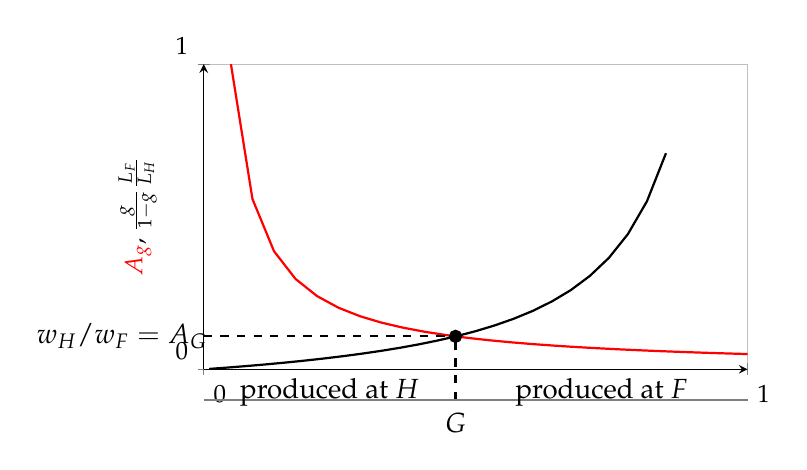
\begin{tikzpicture}
            \begin{axis}[
                axis lines=left,
                xmin=0, xmax=1,
                ymin=0, ymax=1,
                ylabel={\textcolor{red}{$A_g$}, $\frac{g}{1-g} \frac{L_F}{L_H}$},
                xtick={0,1},
                ytick={0,1},
                xticklabels={0, 1},
                xticklabel style={anchor=north west, yshift=0pt},
                yticklabel style={anchor=south east, xshift=0pt},
                enlargelimits=false,
                clip=false,
                grid=major,
                width=12cm,
                height=8cm,
                every axis plot/.style={thick},
                width=0.7\textwidth,
                height=0.45\textwidth,
                label style={font=\small},
                tick label style={font=\small},
            ]
                       
            \pgfmathsetmacro{\z}{0.05}       
            \pgfmathsetmacro{\c}{0.125}         
            \pgfmathsetmacro{\x}{ (-\z + sqrt(\z^2 + 4*\c*\z)) / (2*\c) }
            \pgfmathsetmacro{\y}{ \z / \x  }         
            \addplot[red, thick, domain=0.05:1] {\z / x}; % A_g
            \addplot[black, thick, domain=0.01:0.85] {x / (1 - x) * \c}; % omega(g)
            
            \addplot[dashed] coordinates {(0,\y) (\x,\y)};
            \node at (axis cs:-0.15,\y) {$w_H/w_F=A_G$};
            \addplot[dashed] coordinates {(\x,-.1) (\x,\y)};
            \node at (axis cs:\x,-0.175) {$G$};
            \addplot[gray] coordinates {(0,-0.1) (\x,-0.1)};
            \node at (axis cs:\x/2,-0.075) {produced at $H$};
            \addplot[gray] coordinates {(\x,-0.1) (1,-0.1)};
            \node at (axis cs:( {\x + (1-\x)/2},-0.075) {produced at $F$};
            
            \addplot[only marks, mark=*, color=black, mark size=2pt] coordinates {(\x, \y)};

            \end{axis}
            \end{tikzpicture}
        \caption{Relative unit labor costs and specialization patterns.}
        \label{fig: Ag}
    \end{figure}

\part What happens if the foreign population increases to $L_F'>L_F$?

\textcolor{red}{(i) Home now specializes on a smaller share of goods, only those it is most productive in; and (ii) the relative equilibrium wage increases (home is now relatively wealthier).}

    \begin{figure}[hpd]
        \centering
        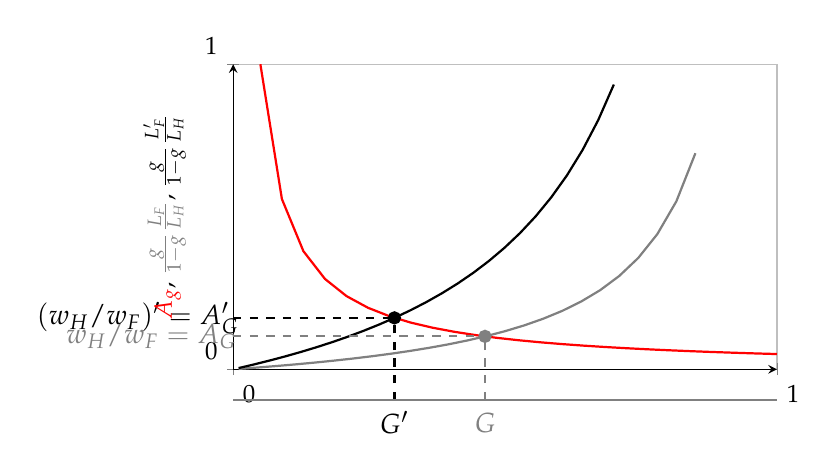
\begin{tikzpicture}
            \begin{axis}[
                axis lines=left,
                xmin=0, xmax=1,
                ymin=0, ymax=1,
                ylabel={\textcolor{red}{$A_g$}, \textcolor{gray}{$\frac{g}{1-g} \frac{L_F}{L_H}$}, $\frac{g}{1-g} \frac{L_F'}{L_H}$},
                xtick={0,1},
                ytick={0,1},
                xticklabels={0, 1},
                xticklabel style={anchor=north west, yshift=0pt},
                yticklabel style={anchor=south east, xshift=0pt},
                enlargelimits=false,
                clip=false,
                grid=major,
                width=12cm,
                height=8cm,
                every axis plot/.style={thick},
                width=0.7\textwidth,
                height=0.45\textwidth,
                label style={font=\small},
                tick label style={font=\small},
            ]
                       
            \pgfmathsetmacro{\z}{0.05}       
            \pgfmathsetmacro{\c}{0.125}         
            \pgfmathsetmacro{\x}{ (-\z + sqrt(\z^2 + 4*\c*\z)) / (2*\c) }
            \pgfmathsetmacro{\y}{ \z / \x  }         
            \addplot[red, thick, domain=0.05:1] {\z / x}; % A_g
            \addplot[gray, thick, domain=0.01:0.85] {x / (1 - x) * \c}; % omega(g)

            \pgfmathsetmacro{\zn}{0.05}       
            \pgfmathsetmacro{\cn}{0.4}         
            \pgfmathsetmacro{\xn}{ (-\zn + sqrt(\zn^2 + 4*\cn*\zn)) / (2*\cn) }
            \pgfmathsetmacro{\yn}{ \zn / \xn  }         
            \addplot[black, thick, domain=0.01:0.7] {x / (1 - x) * \cn}; % omega(g)

            \addplot[dashed, gray] coordinates {(0,\y) (\x,\y)};
            \node[gray] at (axis cs:-0.15,\y) {$w_H/w_F=A_G$};
            \addplot[dashed, gray] coordinates {(\x,-.1) (\x,\y)};
            \node[gray] at (axis cs:\x,-0.175) {$G$};
            \addplot[only marks, mark=*, color=gray, mark size=2pt] coordinates {(\x, \y)};


            \addplot[dashed] coordinates {(0,\yn) (\xn,\yn)};
            \node at (axis cs:-0.175,\yn) {$(w_H/w_F)'=A'_G$};
            \addplot[dashed] coordinates {(\xn,-.1) (\xn,\yn)};
            \node at (axis cs:\xn,-0.175) {$G'$};
            \addplot[gray] coordinates {(0,-0.1) (\xn,-0.1)};
            \addplot[gray] coordinates {(\xn,-0.1) (1,-0.1)};
            \addplot[only marks, mark=*, color=black, mark size=2pt] coordinates {(\xn, \yn)};
            

            \end{axis}
            \end{tikzpicture}
        \caption{Change in relative wages curve}
        \label{fig: Ag-change}
    \end{figure}


\end{parts}

\question Let $F(K,L)$ be a the Cobb-Douglas production function and $0 < \beta < 1$. 

\begin{parts}
    \part Write down the Cobb-Douglas production function.
    \begin{equation*}
        \textcolor{red}{ F(K,L) = \bar{Z} K^{\beta} L^{1-\beta} \qquad \text{ for }  0 < \bar{Z} < \infty \text{, including } \bar{A} = 1}   
    \end{equation*}
        
    \part Prove mathematically that the Cobb-Douglas production function is Constant Returns to Scale (5 pts) and explain with words what it means for a production function to be constant returns to scale (5 pts).

    \textcolor{red}{A constant returns to scale production function means that if you proportionally increase all factors of production you will proportionally increase output, as if you could simply replicate the technology you currently without any loss or gain in efficiency.}

    Proof:

    \begin{align*}
        \textcolor{red}{F(\lambda K,\lambda L)} = \textcolor{red}{\bar{Z}(\lambda K)^\beta (\lambda L)^{1-\beta}}   = \textcolor{red}{\lambda \bar{Z} (K)^\beta (L)^{1-\beta}} = \textcolor{red}{\lambda F(K,L)}
    \end{align*}
    
    \part Write down the firm's profit maximization problem in the Production Model for a firm whose technology is Cobb-Douglas. Make sure to specify choice variables that the firm adjusts in order to maximize profits under the $\max$ operator. Alternatively, if you do not remember how to set up the problem, describe in words the positive flows, negative flows, and choices of this problem.

    \textcolor{red}{\begin{equation*}
        \max_{K,L} \pi = \max_{K,L} \underbrace{P \bar{Z} K^\beta L^{1-\beta}}_{\text{revenues}} - \underbrace{\left( w L + r K \right)}_{\text{costs}}, \text{ also valid normalizing } P = 1
    \end{equation*}}

    \textcolor{red}{The firm chooses capital and labor to maximize its profits, defined as the difference between total revenue (total value of production) and total costs (total wages paid and total rents paid).}

    \part Define the marginal product of labor (MPL) and, using the production function above, show that MPL is decreasing in labor.

    \textcolor{red}{MPL = $\partial Y/\partial L$}

    \textcolor{red}{
    \begin{equation*}
        \frac{\partial Y}{\partial L} =  \frac{\partial \bar{Z} K^\beta L^{1-\beta}}{\partial L} = (1-\beta) \bar{Z} K^\beta L^{1-\beta-1} =  (1-\beta) \bar{Z}  \left( \frac{K}{L} \right)^{\beta}
    \end{equation*}    
    }

    \part Draw the chart of Y as a function of L, holding K fixed. Explain the shape of the chart and state an economic concept that it relates to.

    
    \begin{tikzpicture}
    \pgfmathsetmacro{\alpha}{1/3}    % preference for computers
    \pgfmathsetmacro{\K}{1}    % labor endowment
    \pgfmathsetmacro{\A}{1}    % labor endowment
    
    \centering
    \begin{axis}[
        ylabel={$Y = Z \times K^{\beta} L^{1-\beta}$ },
        xlabel={Used labor input: $L$},
        ymin=0, ymax=5,
        xmin=0, xmax=5,
        yticklabel=\empty,
        xticklabel=\empty,
        axis lines=left,
        enlargelimits=false,
        clip=false,
        axis on top,
        scaled x ticks=false,
        width=9cm, height=7cm,
        title style={font=\bfseries}
    ]
    
    % PPF: Q_C = (L/a_C) - (a_R/a_C) * Q_R
    \addplot[thick, red, domain=0:4] {\A*\K^(\alpha)*x^(1-\alpha)};
    
    \addplot[dashed, gray] coordinates {(0,{\A*\K^(\alpha)*1^(1-\alpha)}) (1,{\A*\K^(\alpha)*1^(1-\alpha)})};
    \addplot[dashed, gray] coordinates {(1,{\A*\K^(\alpha)*1^(1-\alpha)}) ({\A*\K^(\alpha)*1^(1-\alpha)},0) };
    \addplot[mark=*, only marks, black, mark size=1pt] coordinates {(1, {\A*\K^(\alpha)*1^(1-\alpha)} )};
    
    \addplot[dashed, gray] coordinates {(0,{\A*\K^(\alpha)*2^(1-\alpha)}) (2,{\A*\K^(\alpha)*2^(1-\alpha)})};
    \addplot[dashed, gray] coordinates {(2,{\A*\K^(\alpha)*2^(1-\alpha)}) (2,0)};
    
    \addplot[mark=*, only marks, black, mark size=1pt] coordinates {(2, {\A*\K^(\alpha)*2^(1-\alpha)} )};
    
    \addplot[dashed, gray] coordinates {(0,{\A*\K^(\alpha)*3^(1-\alpha)}) (3,{\A*\K^(\alpha)*3^(1-\alpha)})};
    \addplot[dashed, gray] coordinates {(3,{\A*\K^(\alpha)*3^(1-\alpha)}) (3,0)};
    \addplot[mark=*, only marks, black, mark size=1pt] coordinates {(3, {\A*\K^(\alpha)*3^(1-\alpha)} )};
    
    \addplot[dashed, gray] coordinates {(0,{\A*\K^(\alpha)*4^(1-\alpha)}) (4,{\A*\K^(\alpha)*4^(1-\alpha)})};
    \addplot[dashed, gray] coordinates {(4,{\A*\K^(\alpha)*4^(1-\alpha)}) (4,0)};
    \addplot[mark=*, only marks, black, mark size=1pt] coordinates {(4, {\A*\K^(\alpha)*4^(1-\alpha)} )};
    
    \end{axis}
    
    \end{tikzpicture}

    \textcolor{red}{The "belly shaped" (concave) function relates to diminishing marginal returns. As you hold $K$ fixed an increase $L$, each additional worker adds less to output, because MPL is decreasing in labor.}
    
    \part Derive the optimality conditions for choices $K$ and $L$ in the maximization problem of the firm. Interpret economically what they mean.

    \textcolor{red}{ $\frac{\partial \pi }{\partial K} = 0 \iff P \times \beta \times \bar{Z} \left( \frac{L}{K} \right)^{1-\beta} - r = 0 \implies P \times MPK = r$ }

    \textcolor{red}{ $\frac{\partial \pi }{\partial L} = 0 \iff P \times (1-\beta) \times \bar{Z} \left( \frac{K}{L} \right)^{\beta} - w = 0 \implies P \times MPL = w$ }

    \textcolor{red}{At its optimal choice, factor prices (their marginal costs) equal the marginal revenue they bring to the firm (price times marginal product).}

    \part Suppose that labor supply is $L^S = \bar{L} = 1$ and capital supply is $K^S=\bar{K} = 1$. Using (i) the optimality conditions for the firm, (ii) the production function, (iii) a price normalization of $P=1$, (iv) the values $\bar{Z}=1$ and $\beta=1/2$; (v) and two market clearing conditions, solve for equilibrium prices $(w,r)$ and equilibrium output $Y$.
\textcolor{red}{
    \begin{eqnarray*}
        Y &=& \bar{Z} K^{1/2} L^{1/2} = 1^{1/2} 1^{1/2} = 1 \\
        w &=& \frac{1}{2}\left( \frac{L}{K} \right)^{1/2} = \frac{1}{2}\left( \frac{1}{1} \right)^{1/2} = \frac{1}{2} \\
        r &=& \frac{1}{2}\left( \frac{K}{L} \right)^{1/2} = \frac{1}{2}\left( \frac{1}{1} \right)^{1/2} =\frac{1}{2} \\
        K &=& \bar{K} = 1 \\
        L &=& \bar{L} = 1 
    \end{eqnarray*}
}
    \textcolor{red}{Therefore: $Y = 1$, $(w,r) = (1/2,1/2)$.}

\end{parts}
\end{questions}




\end{document}
